% STEREO
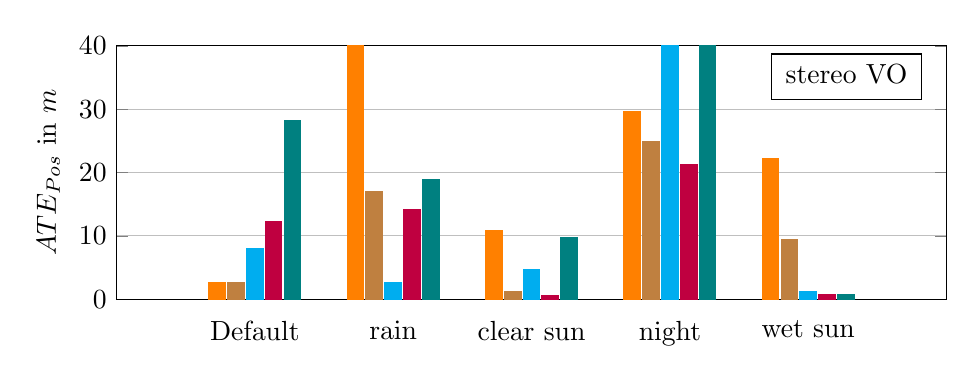
\begin{tikzpicture}
    \begin{axis}[
        width  = \textwidth,
        height = 4.8cm,
        ymax =40,
        major x tick style = transparent,
        ybar=2*\pgflinewidth,
        bar width=6pt,
        ymajorgrids = true,
        ylabel = {$ATE_{Pos}$ in $m$},
        % xlabel = {1 Default, 2 hard rain, 3 clear sunset, 4 clear night ,5 wet sunset},
        symbolic x coords={Default, rain, clear sun, night ,wet sun},
        xtick = data,
        scaled y ticks = false,
        enlarge x limits=0.25,
        ymin=0,
        legend pos=north east
    ]
    \addlegendimage{empty legend}
    \addlegendentry{stereo VO}
    \addplot[style={orange,fill=orange,mark=none}]
        coordinates {(Default, 2.70) (rain,66.61) (clear sun, 10.79) (night ,29.61) (wet sun, 22.271)};
    
    \addplot[style={brown,fill=brown,mark=none}]
        coordinates {(Default, 2.68) (rain,16.94) (clear sun, 1.16) (night , 24.96) (wet sun, 9.48)};
    
    \addplot[style={cyan,fill=cyan,mark=none}]
        coordinates {(Default, 8.07) (rain,2.663) (clear sun, 4.63) (night , 86.94) (wet sun, 1.29)};
    
    \addplot[style={purple,fill=purple,mark=none}]
        coordinates {(Default, 12.2) (rain,14.13) (clear sun, 0.569) (night ,21.32) (wet sun, .7)};
    
    \addplot[style={teal,fill=teal,mark=none}]
        coordinates {(Default, 28.2) (rain,18.87) (clear sun, 9.78) (night ,91.45) (wet sun, .7)};
    \end{axis}
  \end{tikzpicture}